\section{Clase}
\label{sec:clase}
Hasta ahora se fueron definiendo componentes básicos que pertenecen al estándar
UML, específicamente, subcomponentes los cuales definen, como ya se mencionó,
los datos y el comportamiento de los objetos instanciados, ahora, es necesaria
otra entidad que permita la conjunción de estas herramientas, para eso, se
define el componente de \texttt{clase}.

La notación BNF para la definición de una clase en Director es la siguiente:

\begin{lstlisting}[caption={BNF - Clase}, basicstyle=\footnotesize\ttfamily]
  <clase> ::= "class" <nombre> "{" <atributos|metodos> "}"
\end{lstlisting}

Los subcomponentes se trataron en secciones anteriores del documento, de todas
formas se detalla el BNF correspondiente a la pluralización de los mismos.

\begin{lstlisting}[basicstyle=\footnotesize\ttfamily]
  <atributos> ::= <atributo> | <atributos>
\end{lstlisting}

\begin{lstlisting}[basicstyle=\footnotesize\ttfamily]
  <metodos> ::= <metodo> | <metodos>
\end{lstlisting}

Volviendo al ejemplo tratado en la \texttt{Sección \ref{sec:atributo}},
agregando los que se dijo en el \texttt{Fragmento
\ref{lst:drt_java_modelo_metodo_generico}},
se puede completar la consigna juntando los componentes del lenguaje definidos
y ejemplificados anteriormente junto con el elemento que se esta
definiendo aquí en un modelo.

\begin{lstlisting}[caption={Director - Adhiere componente clase al ejemplo},
basicstyle=\footnotesize\ttfamily, label=lst:drt_java_clase]
	class Persona {
		private nombre:string
		private apellido:string
		private DNI:string {@readOnly, @unique}
		public metodo_generico():void
	}
\end{lstlisting}

Lo  cual generaría el siguiente código en un lenguaje como Java:

\begin{lstlisting}[caption={Java - Resultado obtenido de la generación de
\texttt{Fragmento \ref{lst:drt_java_clase}}}, language=Java, basicstyle=\footnotesize\ttfamily]
	class Persona{
		private String nombre;
		private String apellido;
		private String DNI;

		public String get_nombre(){
			return this.nombre;
		}

		public void set_nombre(String nombre){
			this.nombre = nombre;
		}

		public String get_apellido(){
			return this.apellido;
		}

		public void set_apellido(String apellido){
			this.apellido = apellido;
		}

		public String get_DNI(){
			return this.DNI;
		}

		public void set_DNI(String DNI){
			this.DNI = DNI;
		}

		public void metodo_generico() {
			// Implementacion del metodo
		}
	}
\end{lstlisting}

Además es posible su representación mediante el siguiente autómata finito:

\begin{figure}[H]
	\centering
	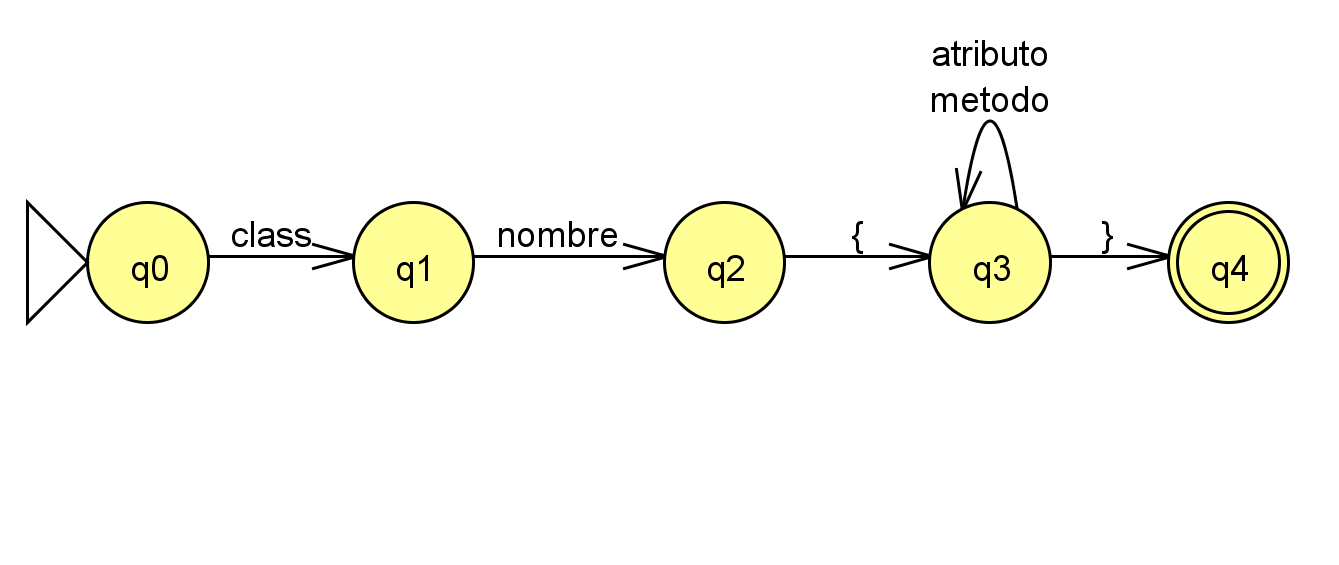
\includegraphics[width=.4\linewidth]{automatas_finitos/classDrt.png}
	\caption{Autómata finito - Clase}
	\label{fig:af_clase}
\end{figure}
